\documentclass[14pt,a4paper,landscape]{article}
\usepackage[utf8]{inputenc}
\usepackage{graphicx}
\usepackage[left=2cm,right=2cm,top=2cm,bottom=2cm]{geometry}
\author{Andrea Colarieti Tosti}
\title{Analysis Blatt 1 Lösung}

\begin{document}
\maketitle
\newpage

\section*{Augabe 1}
Die Mengen-Operationen Schnitt $\cap$  und Vereinigung $\cup$  sind kommutativ, assoziativ und zueinander distributiv.\\
Für die Differenzmenge gelten Assoziativ und Distributivgesetze.

\subsection*{a)}
\begin{center}
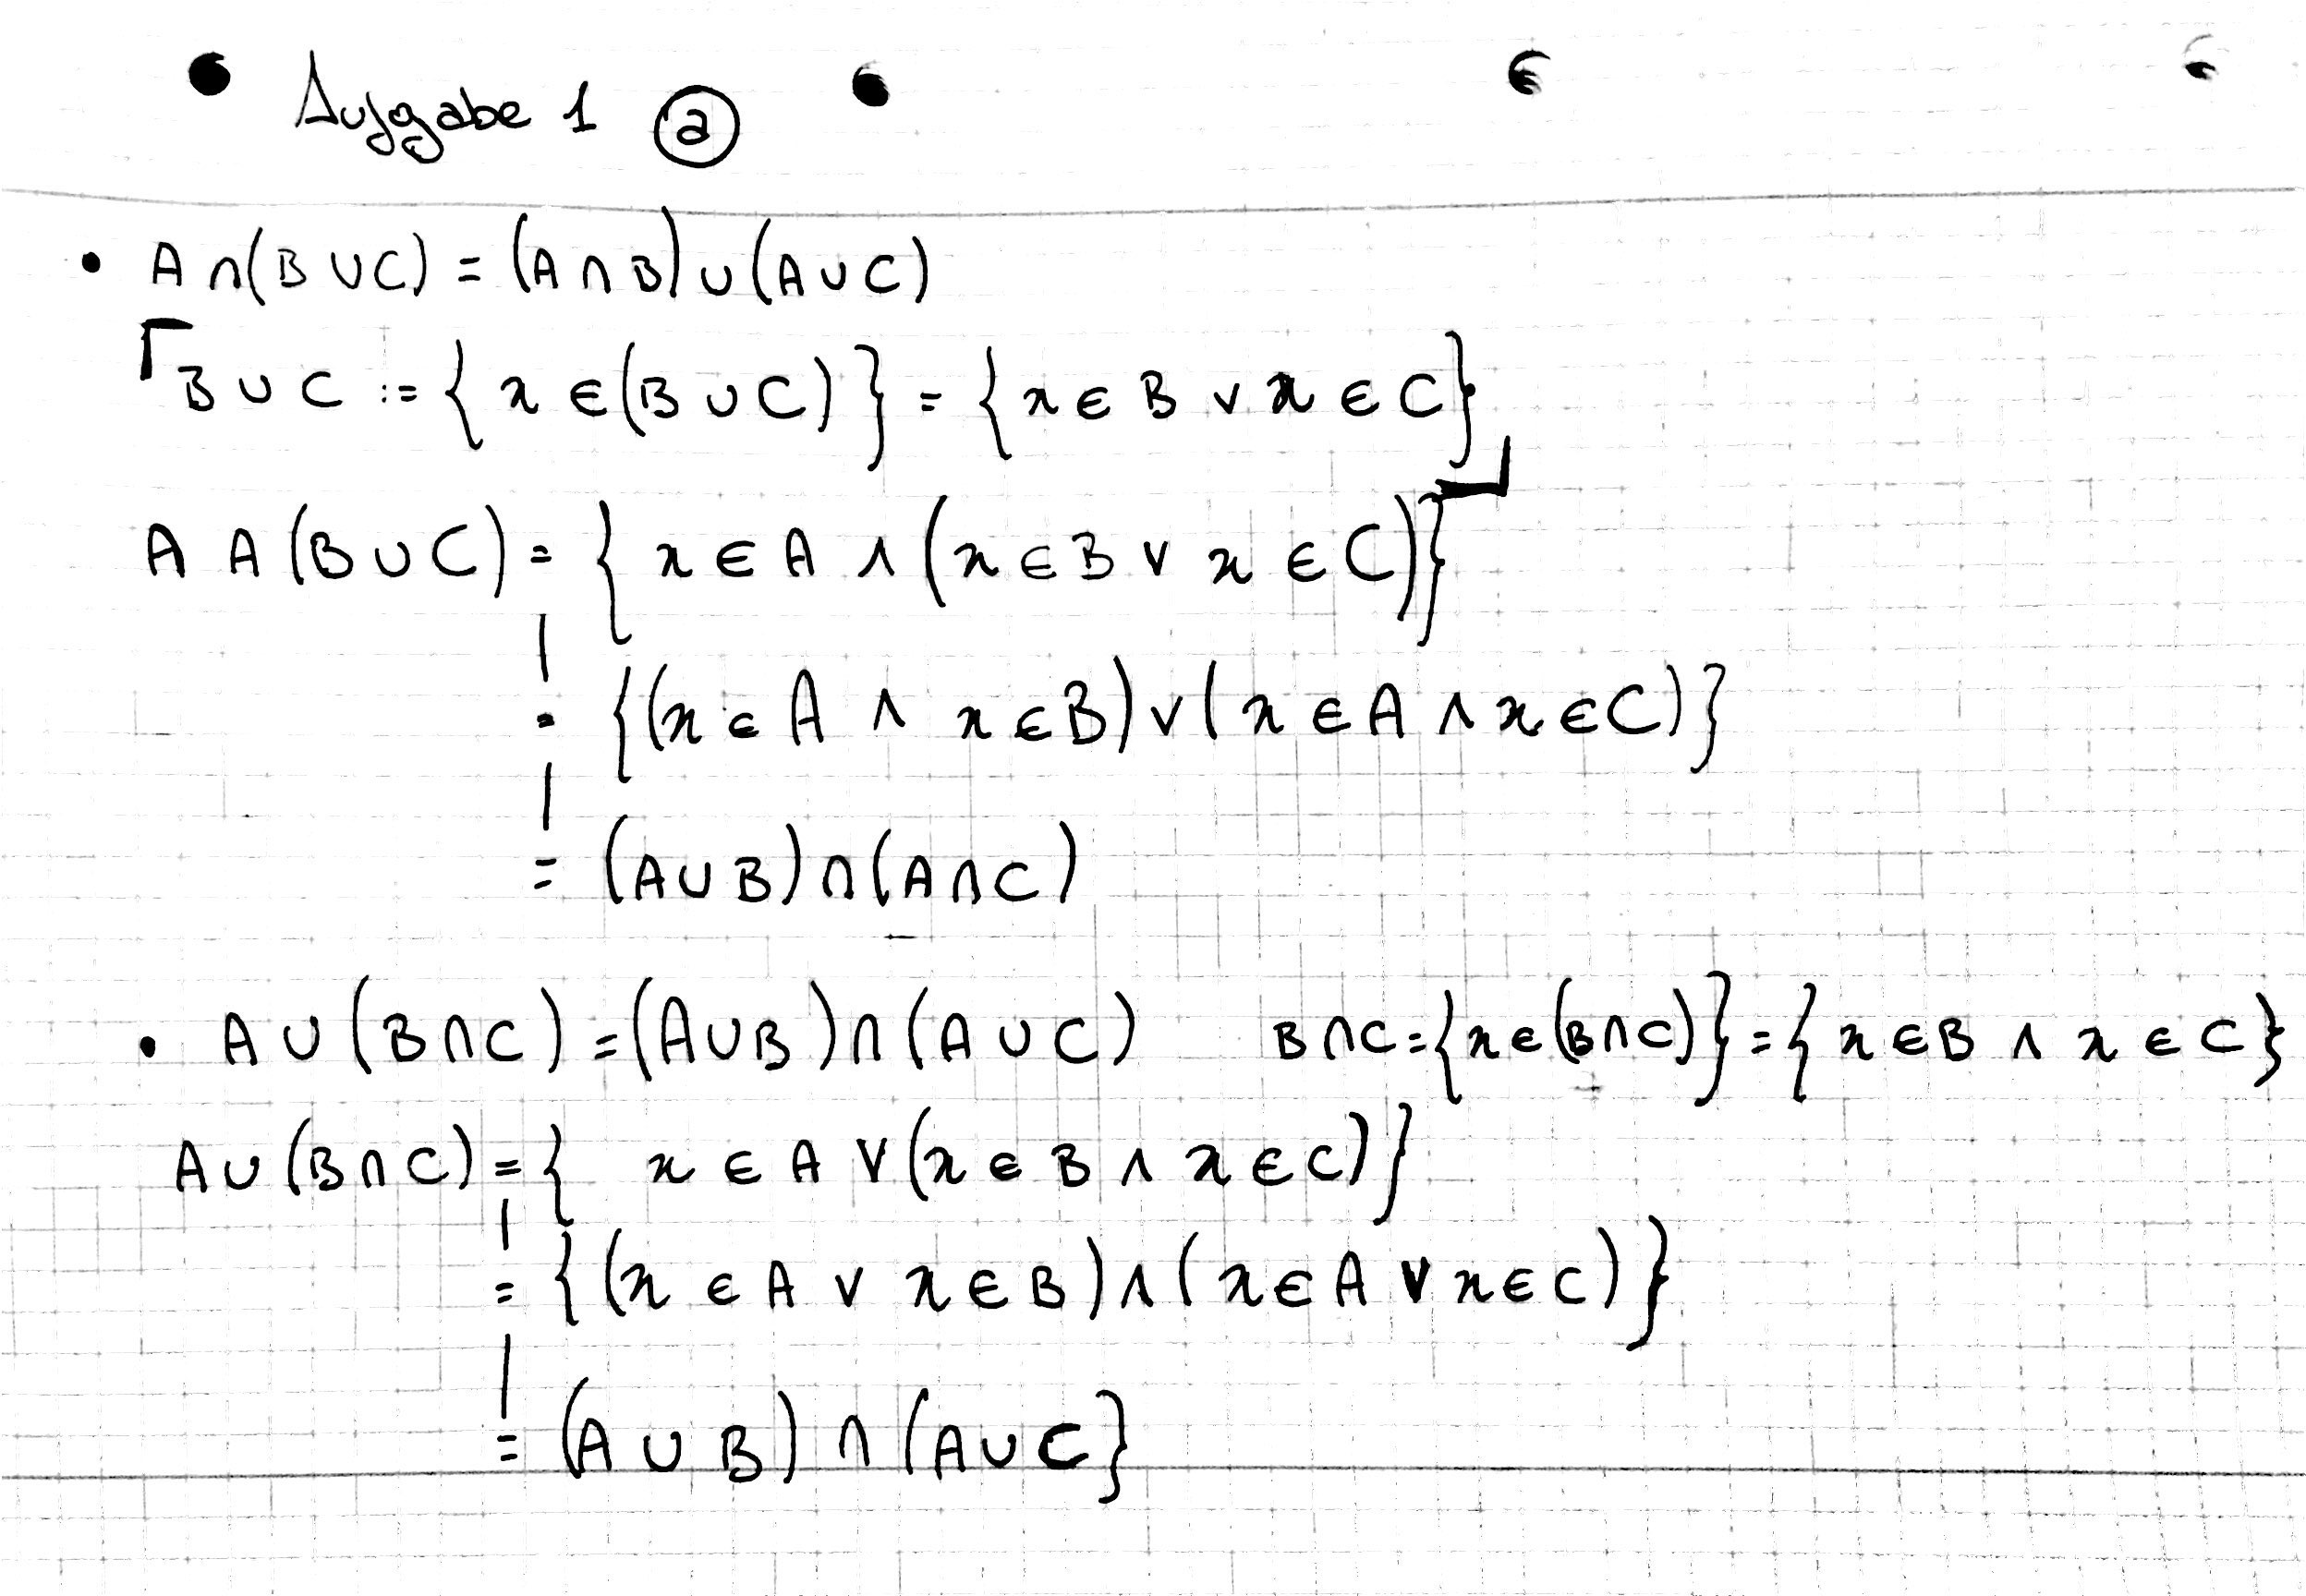
\includegraphics[scale=0.23]{AB1-1_1.jpg} 
\end{center}
\subsection*{b)}
\begin{center}
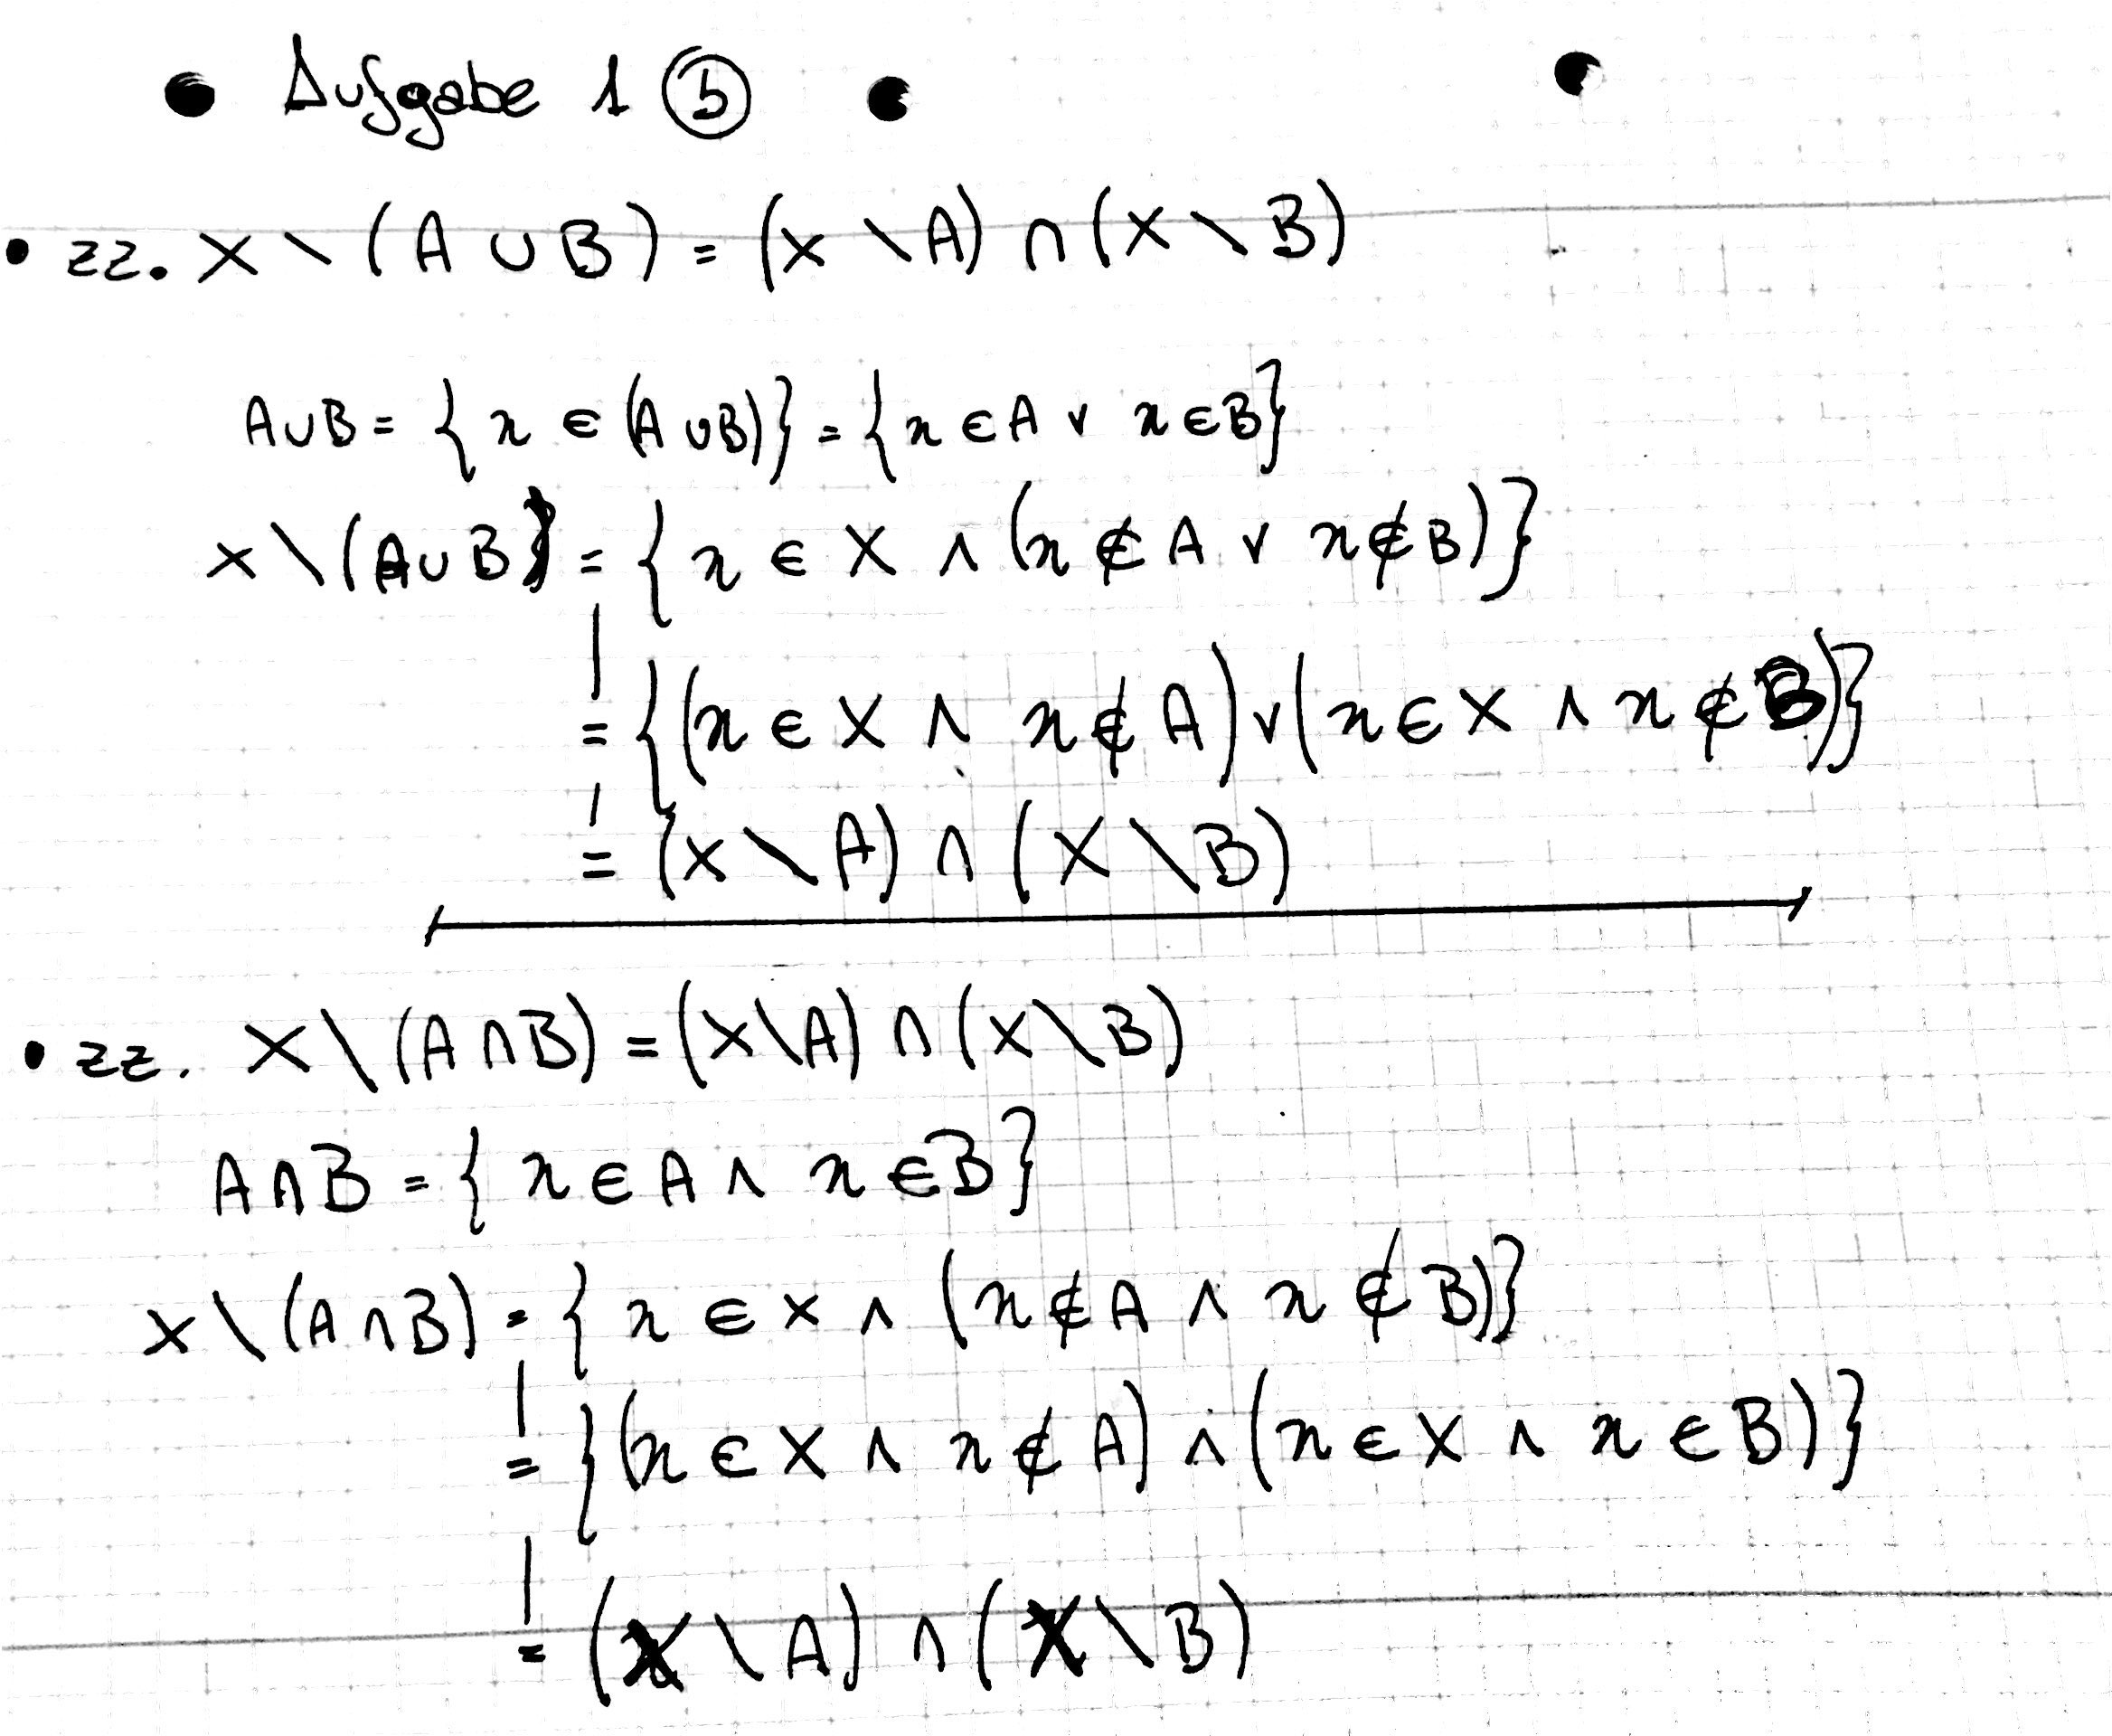
\includegraphics[scale=0.25]{AB1-1_2.jpg} 
\end{center}

\section*{Augabe 2}
\subsection*{a und b}
\begin{center}
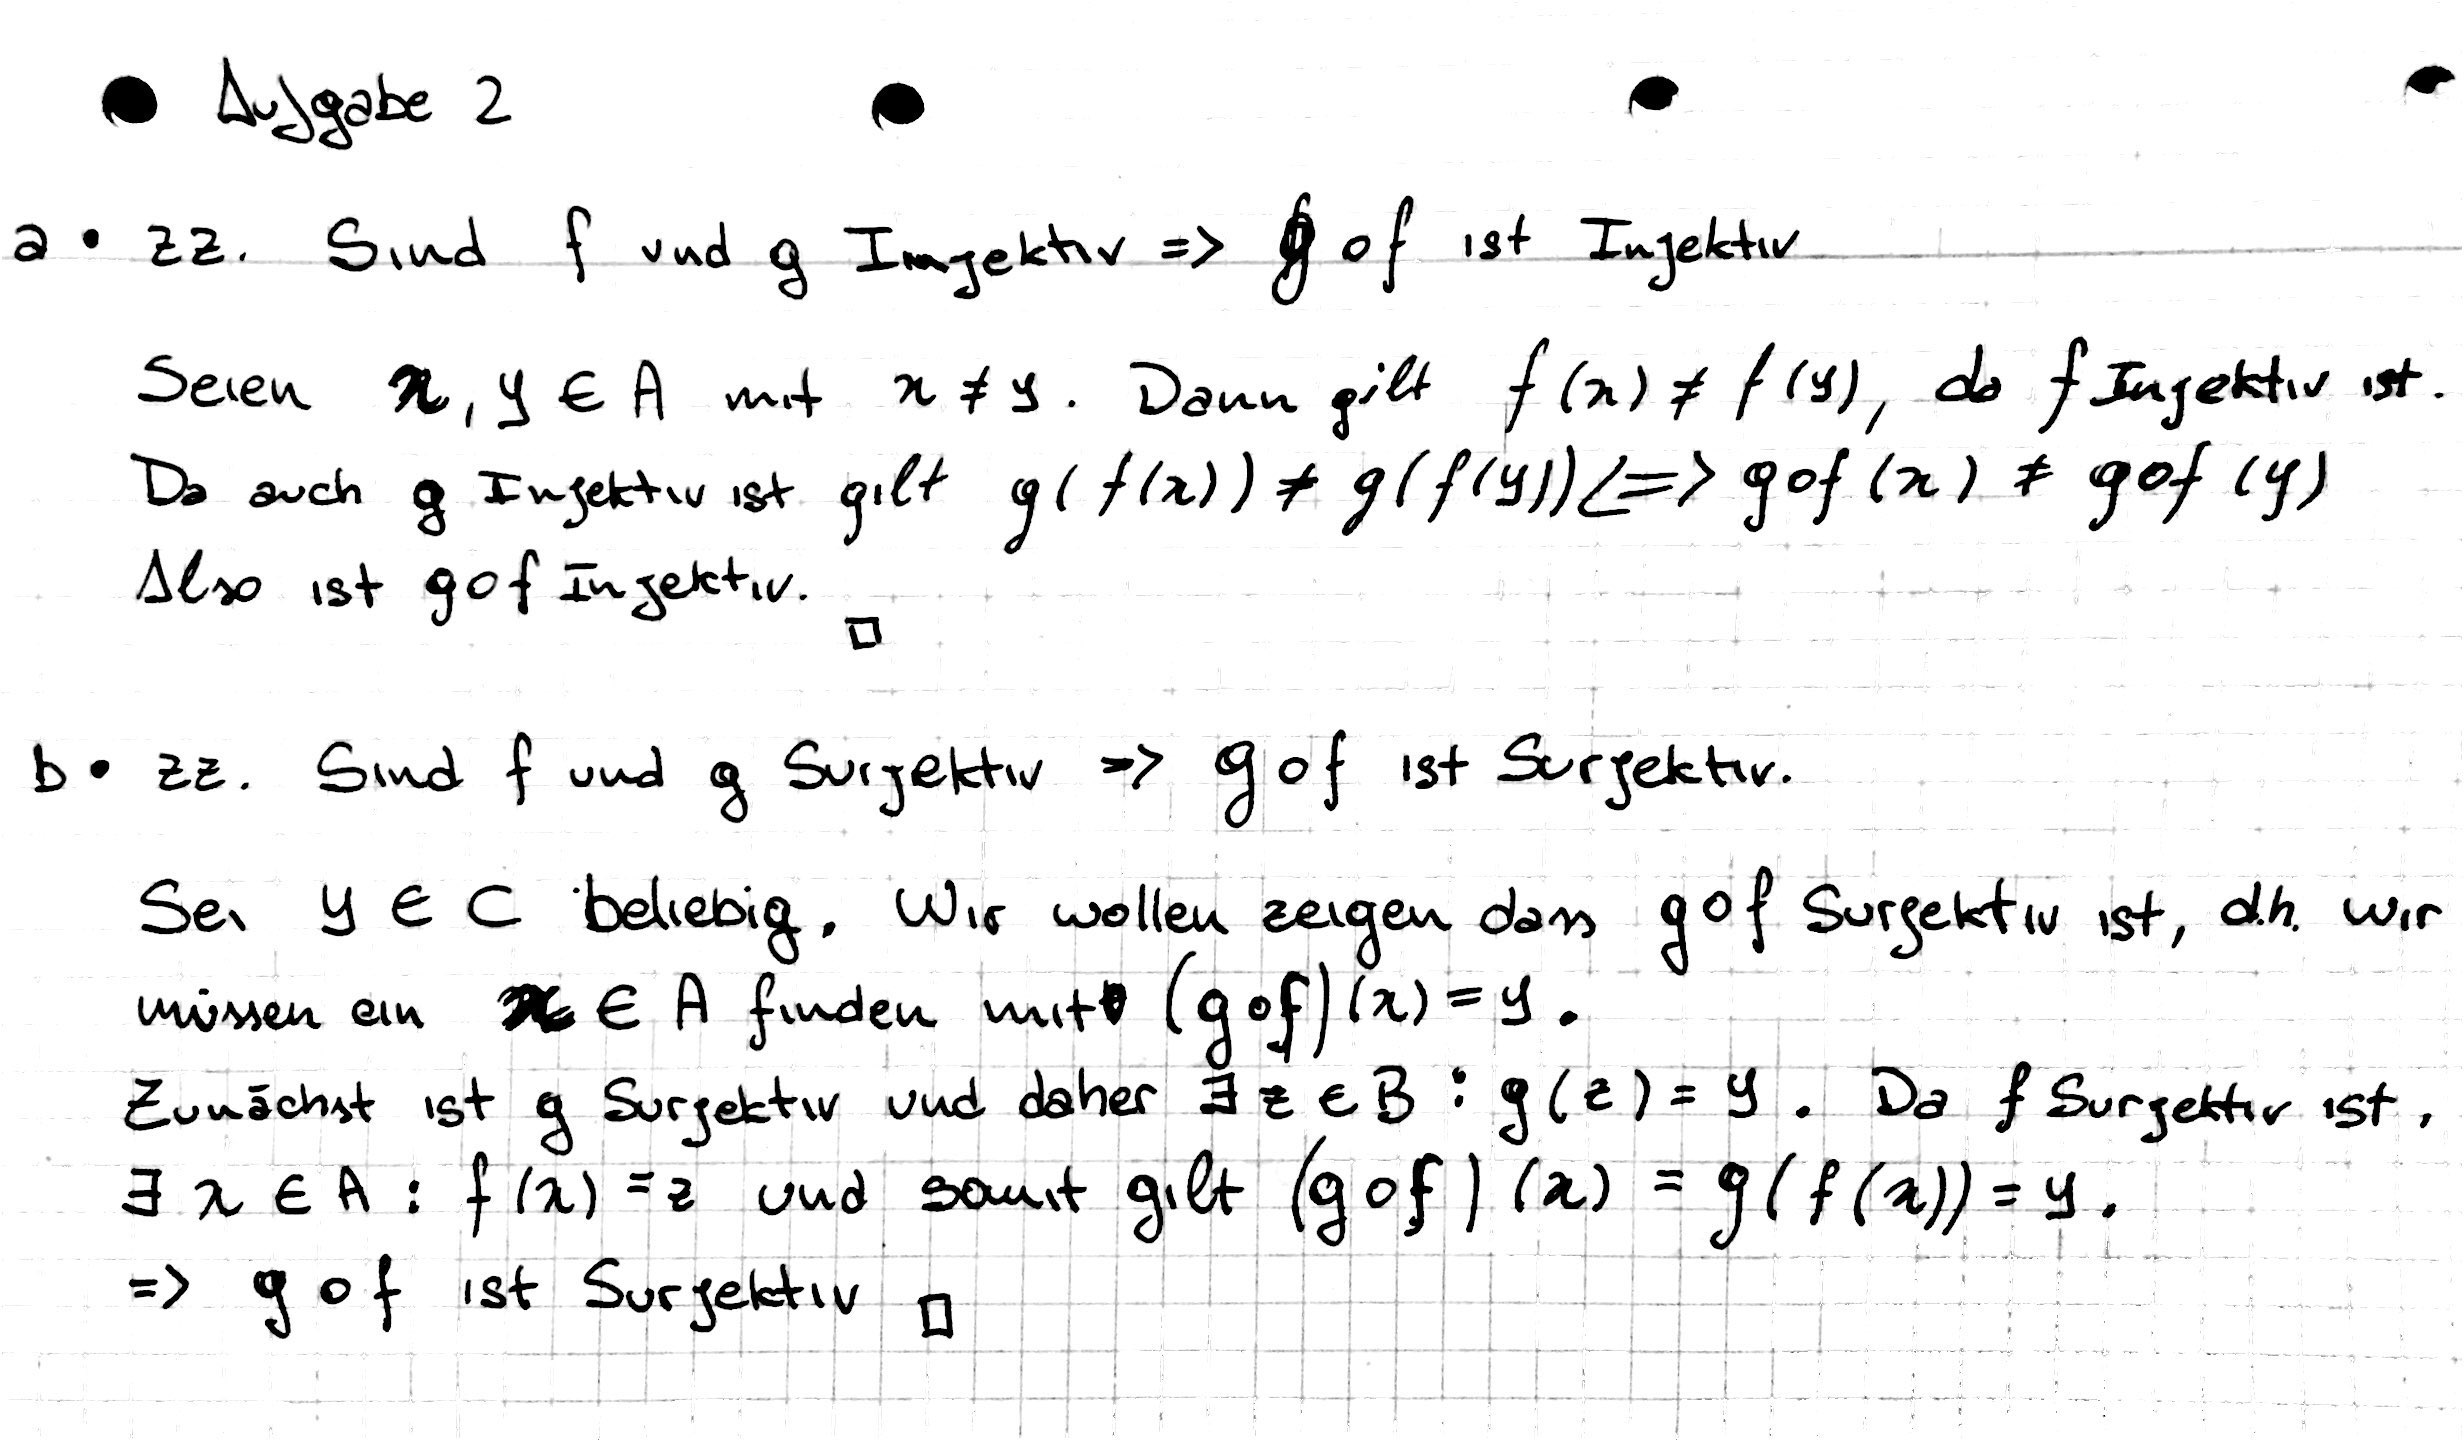
\includegraphics[scale=0.3]{AB1-2_1.jpg} 
\end{center}
\subsection*{c und d}
\begin{center}
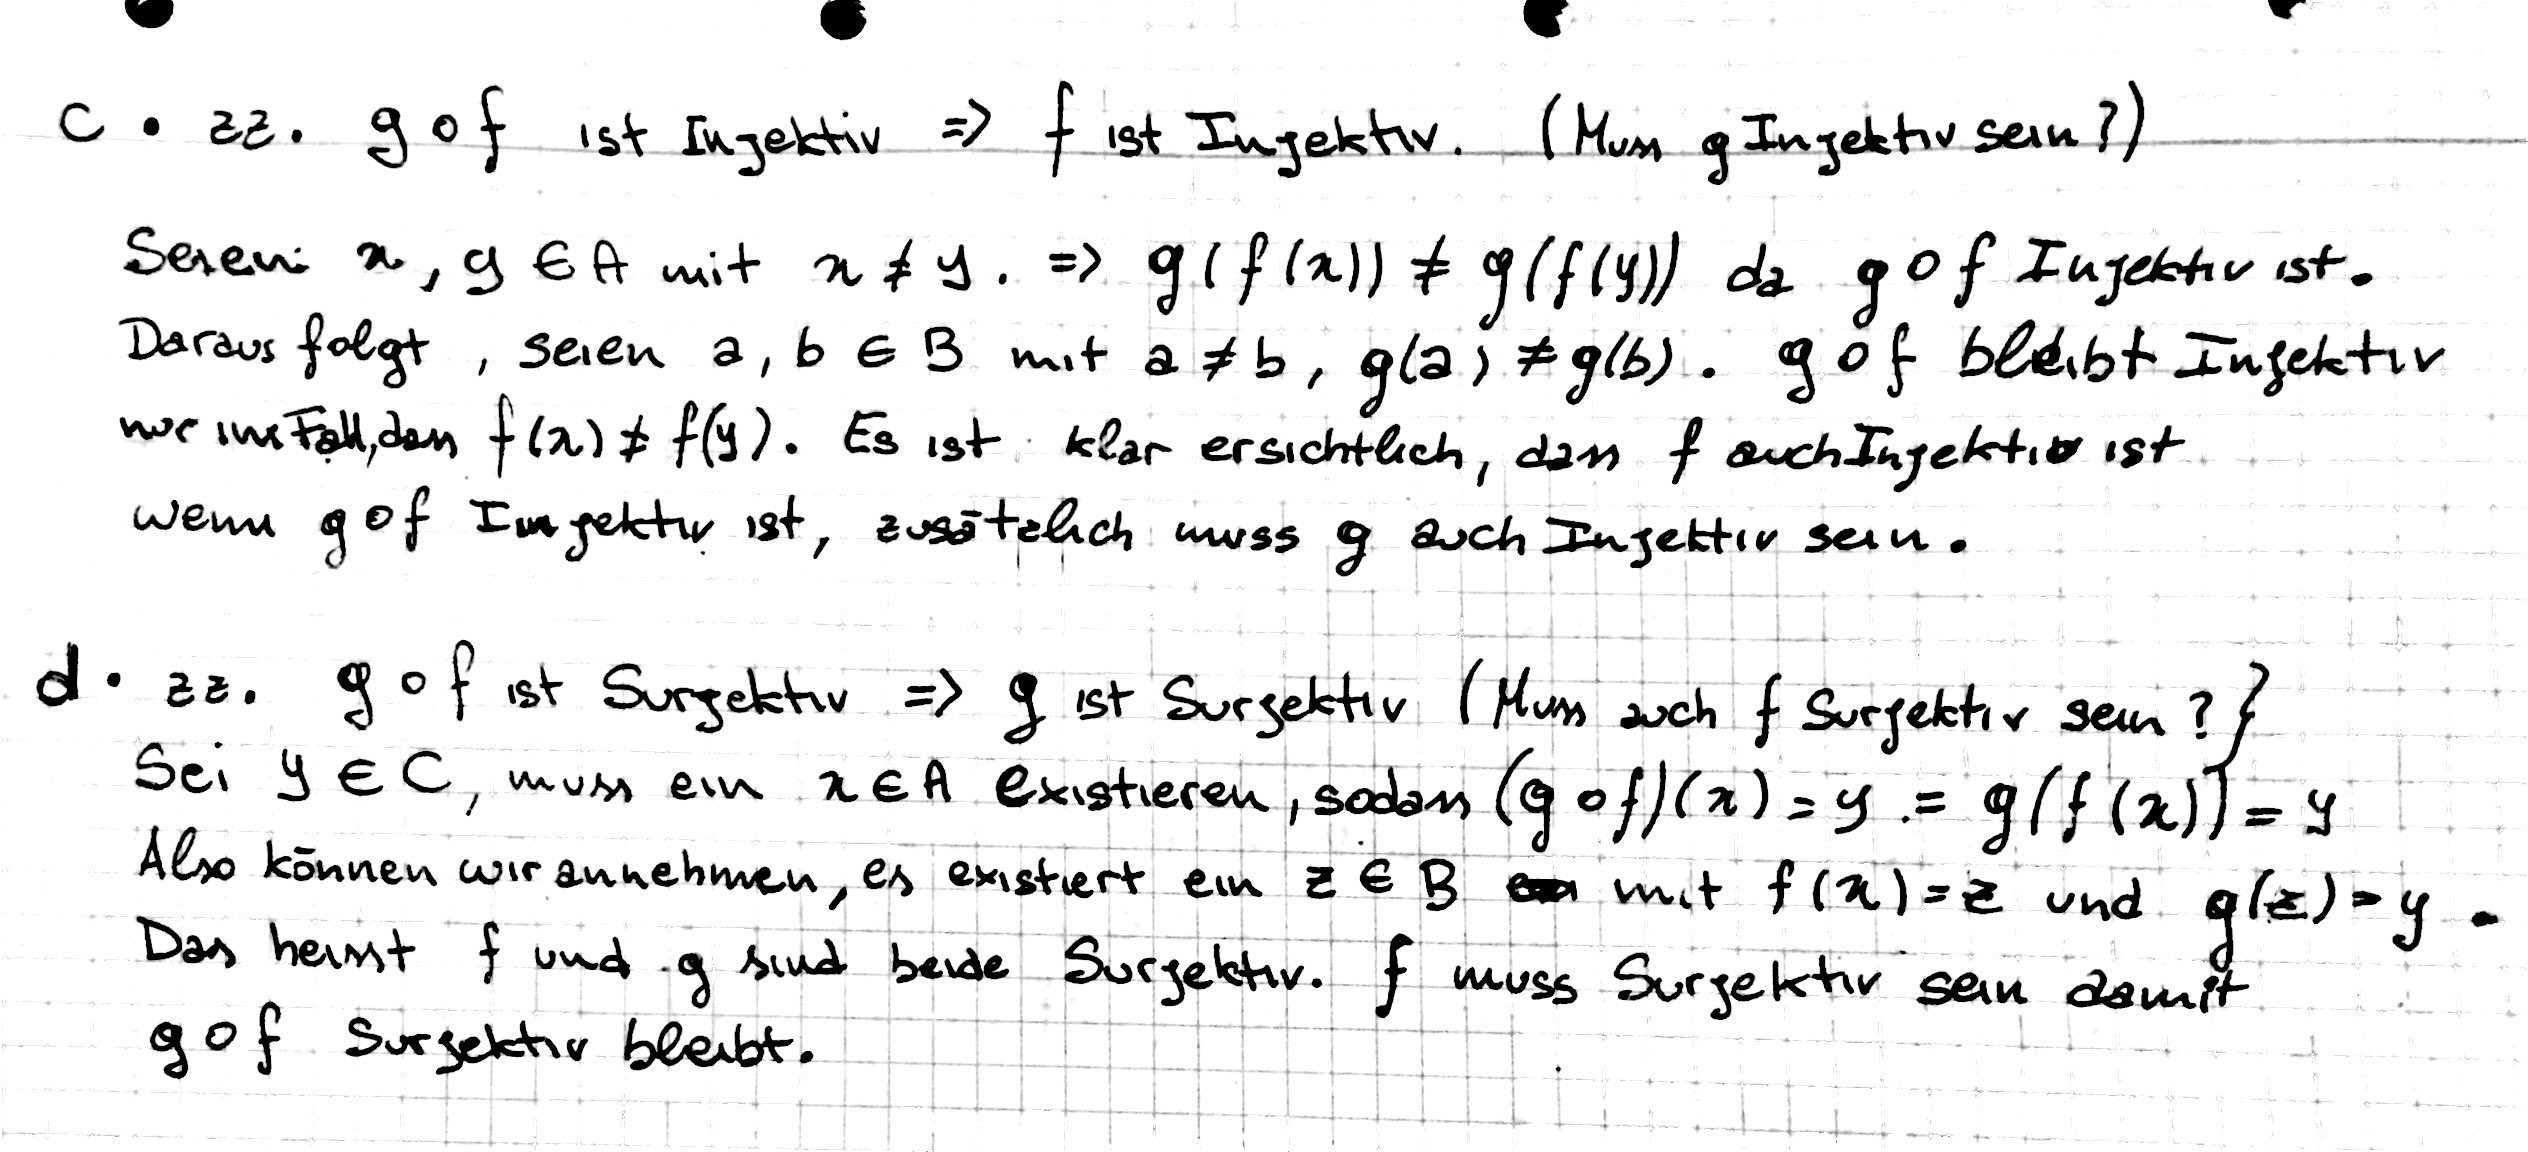
\includegraphics[scale=0.3]{AB1-2_2.jpg} 
\end{center}

\newpage
\section*{Augabe 3}
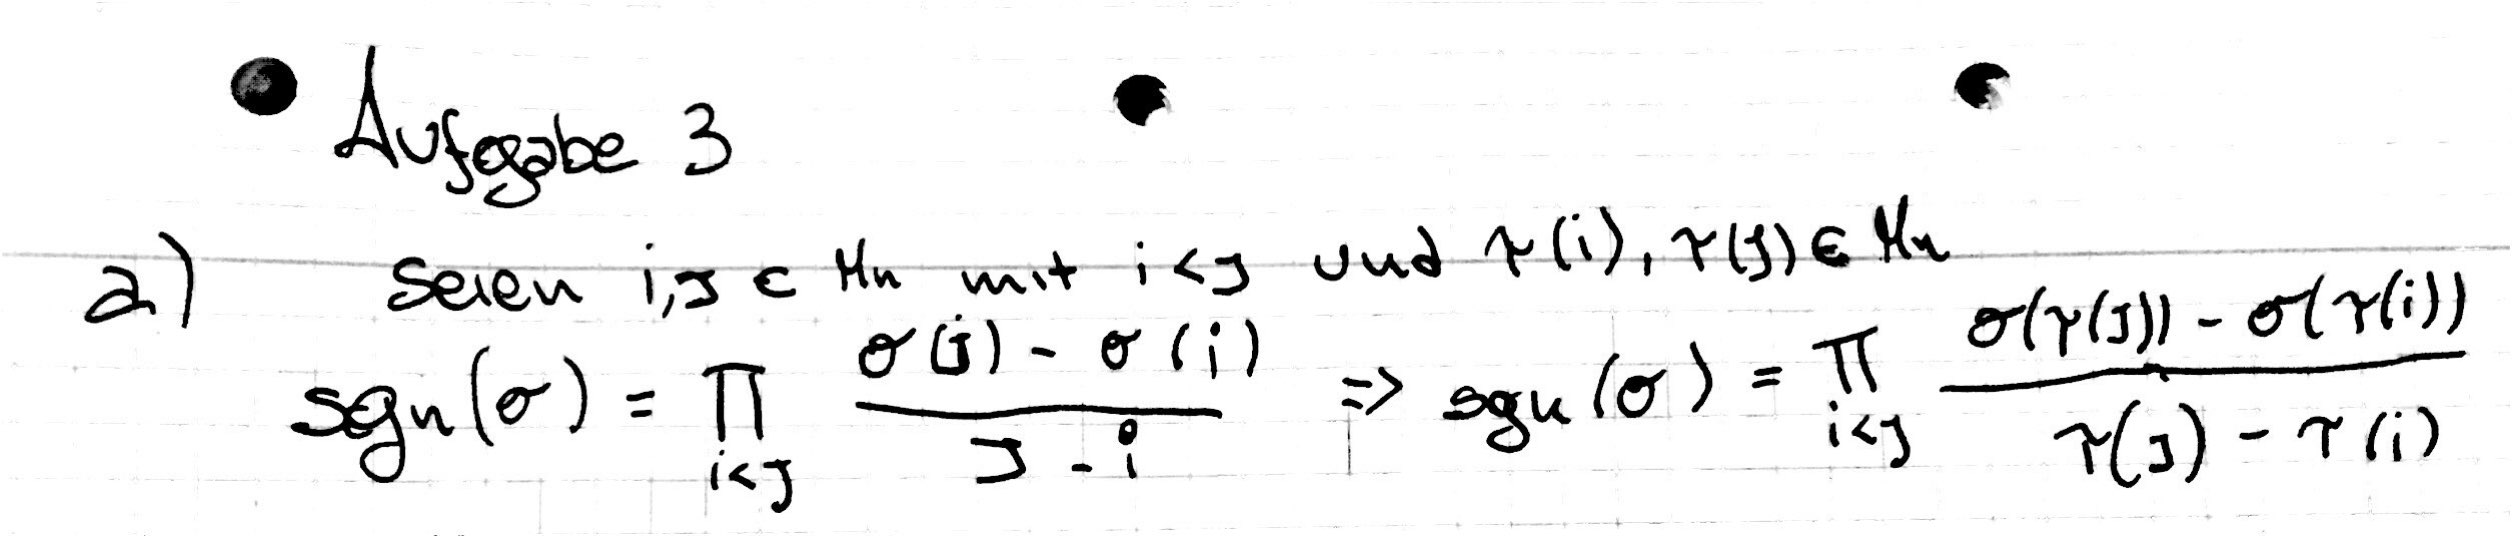
\includegraphics[scale=0.3]{AB1-3_2.jpg} 
\newpage
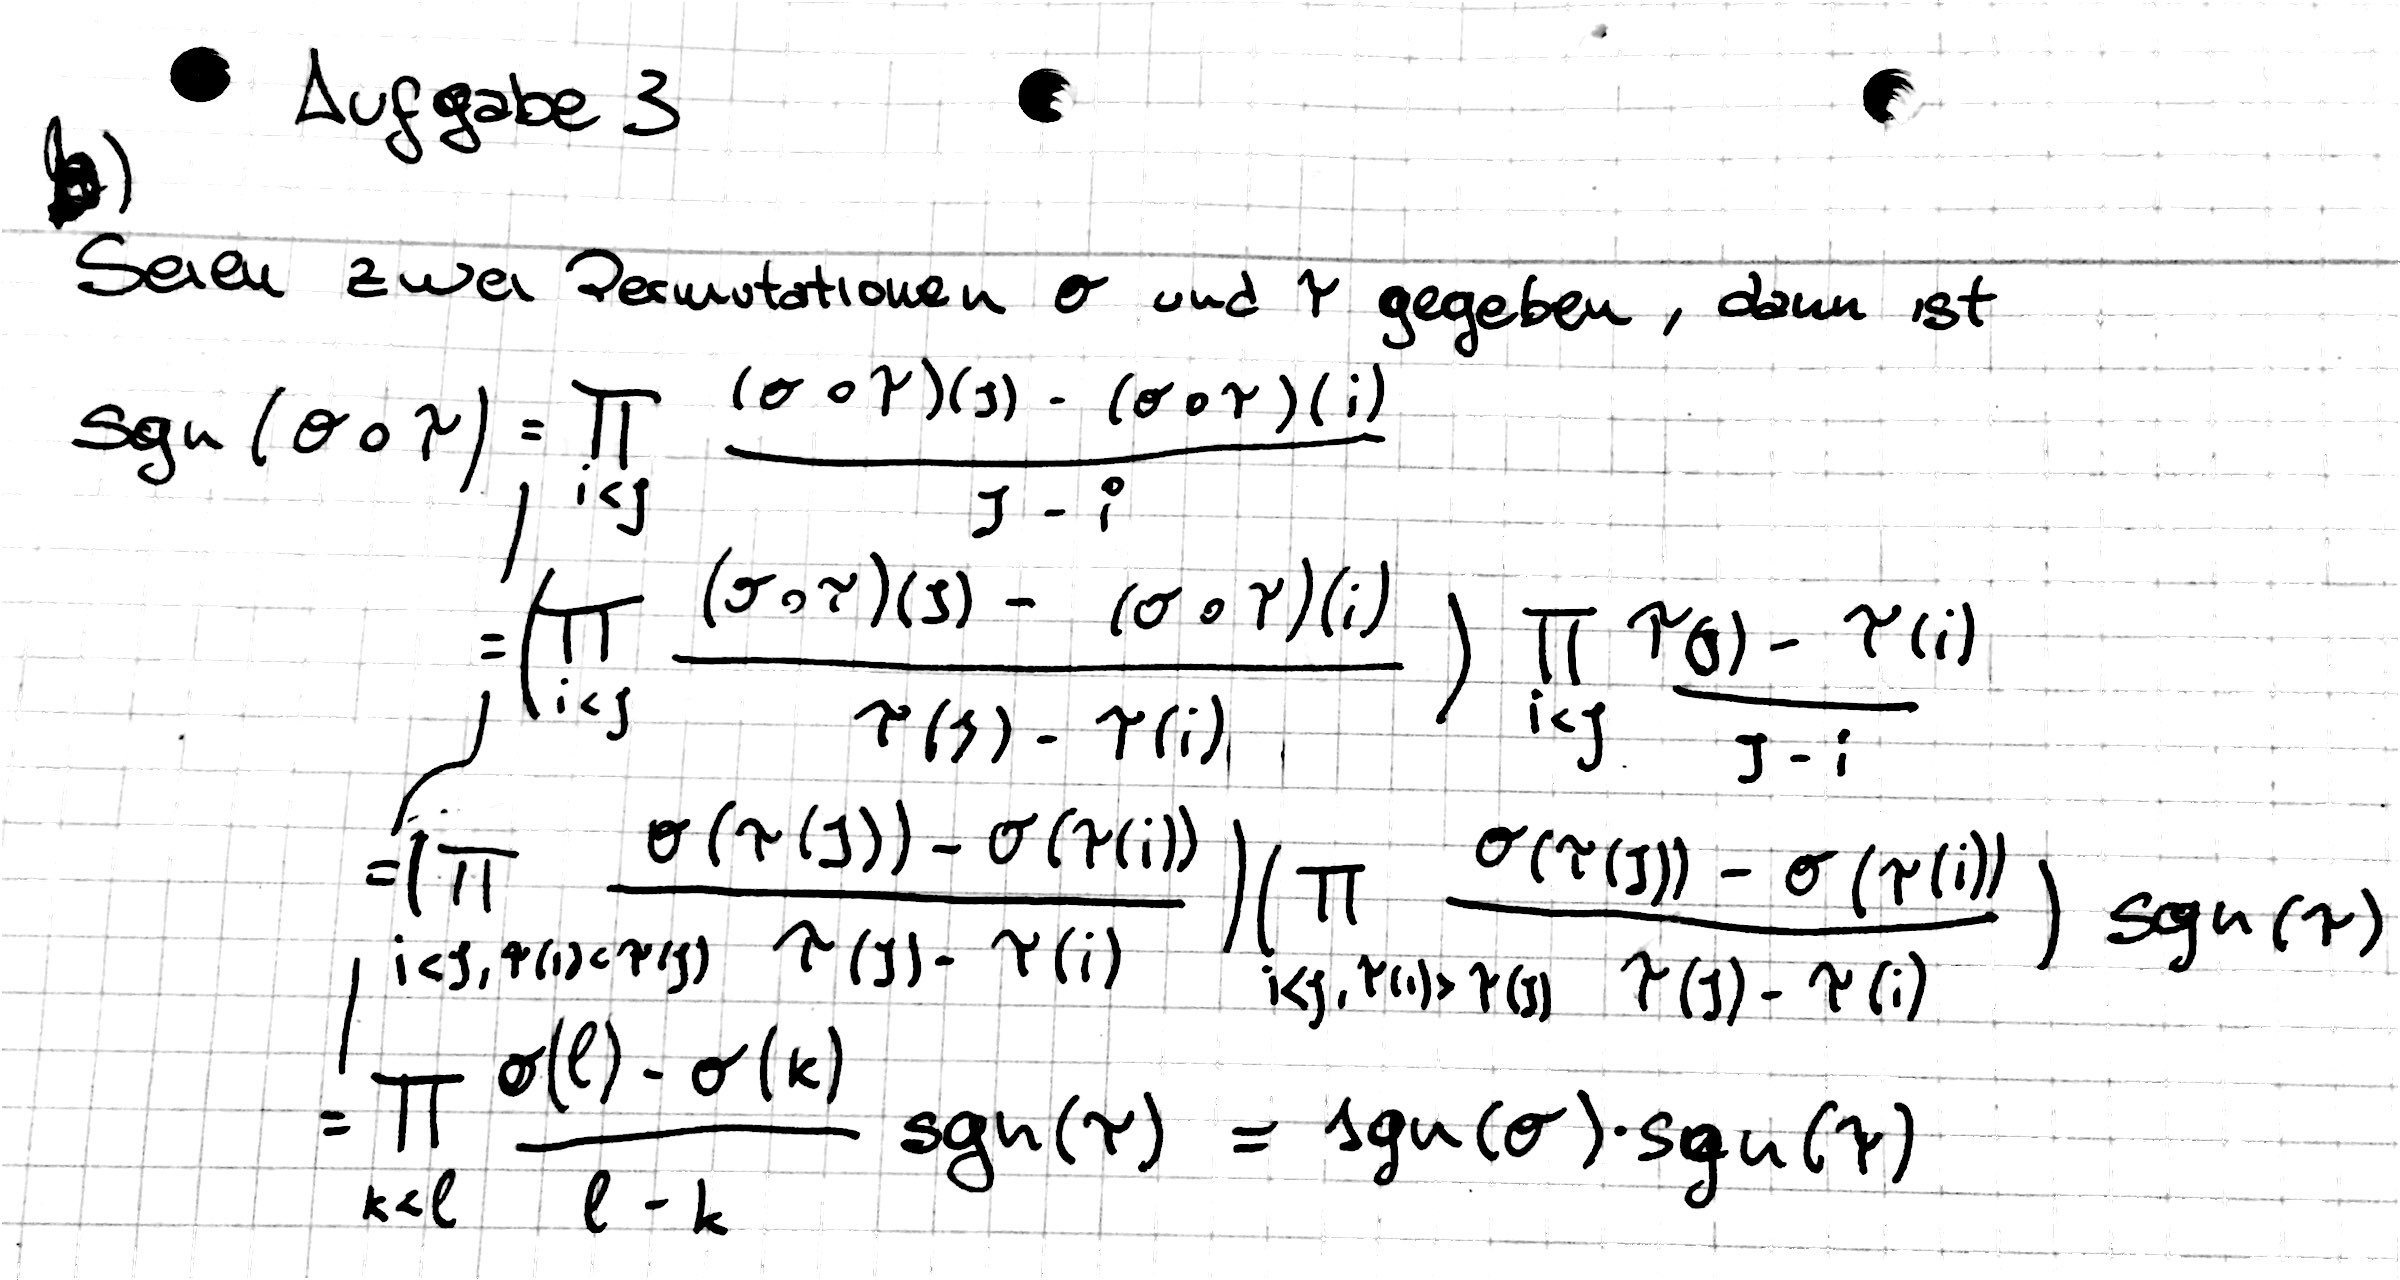
\includegraphics[scale=0.3]{AB1-3_1.jpg} 

\newpage
\section*{Augabe 4}
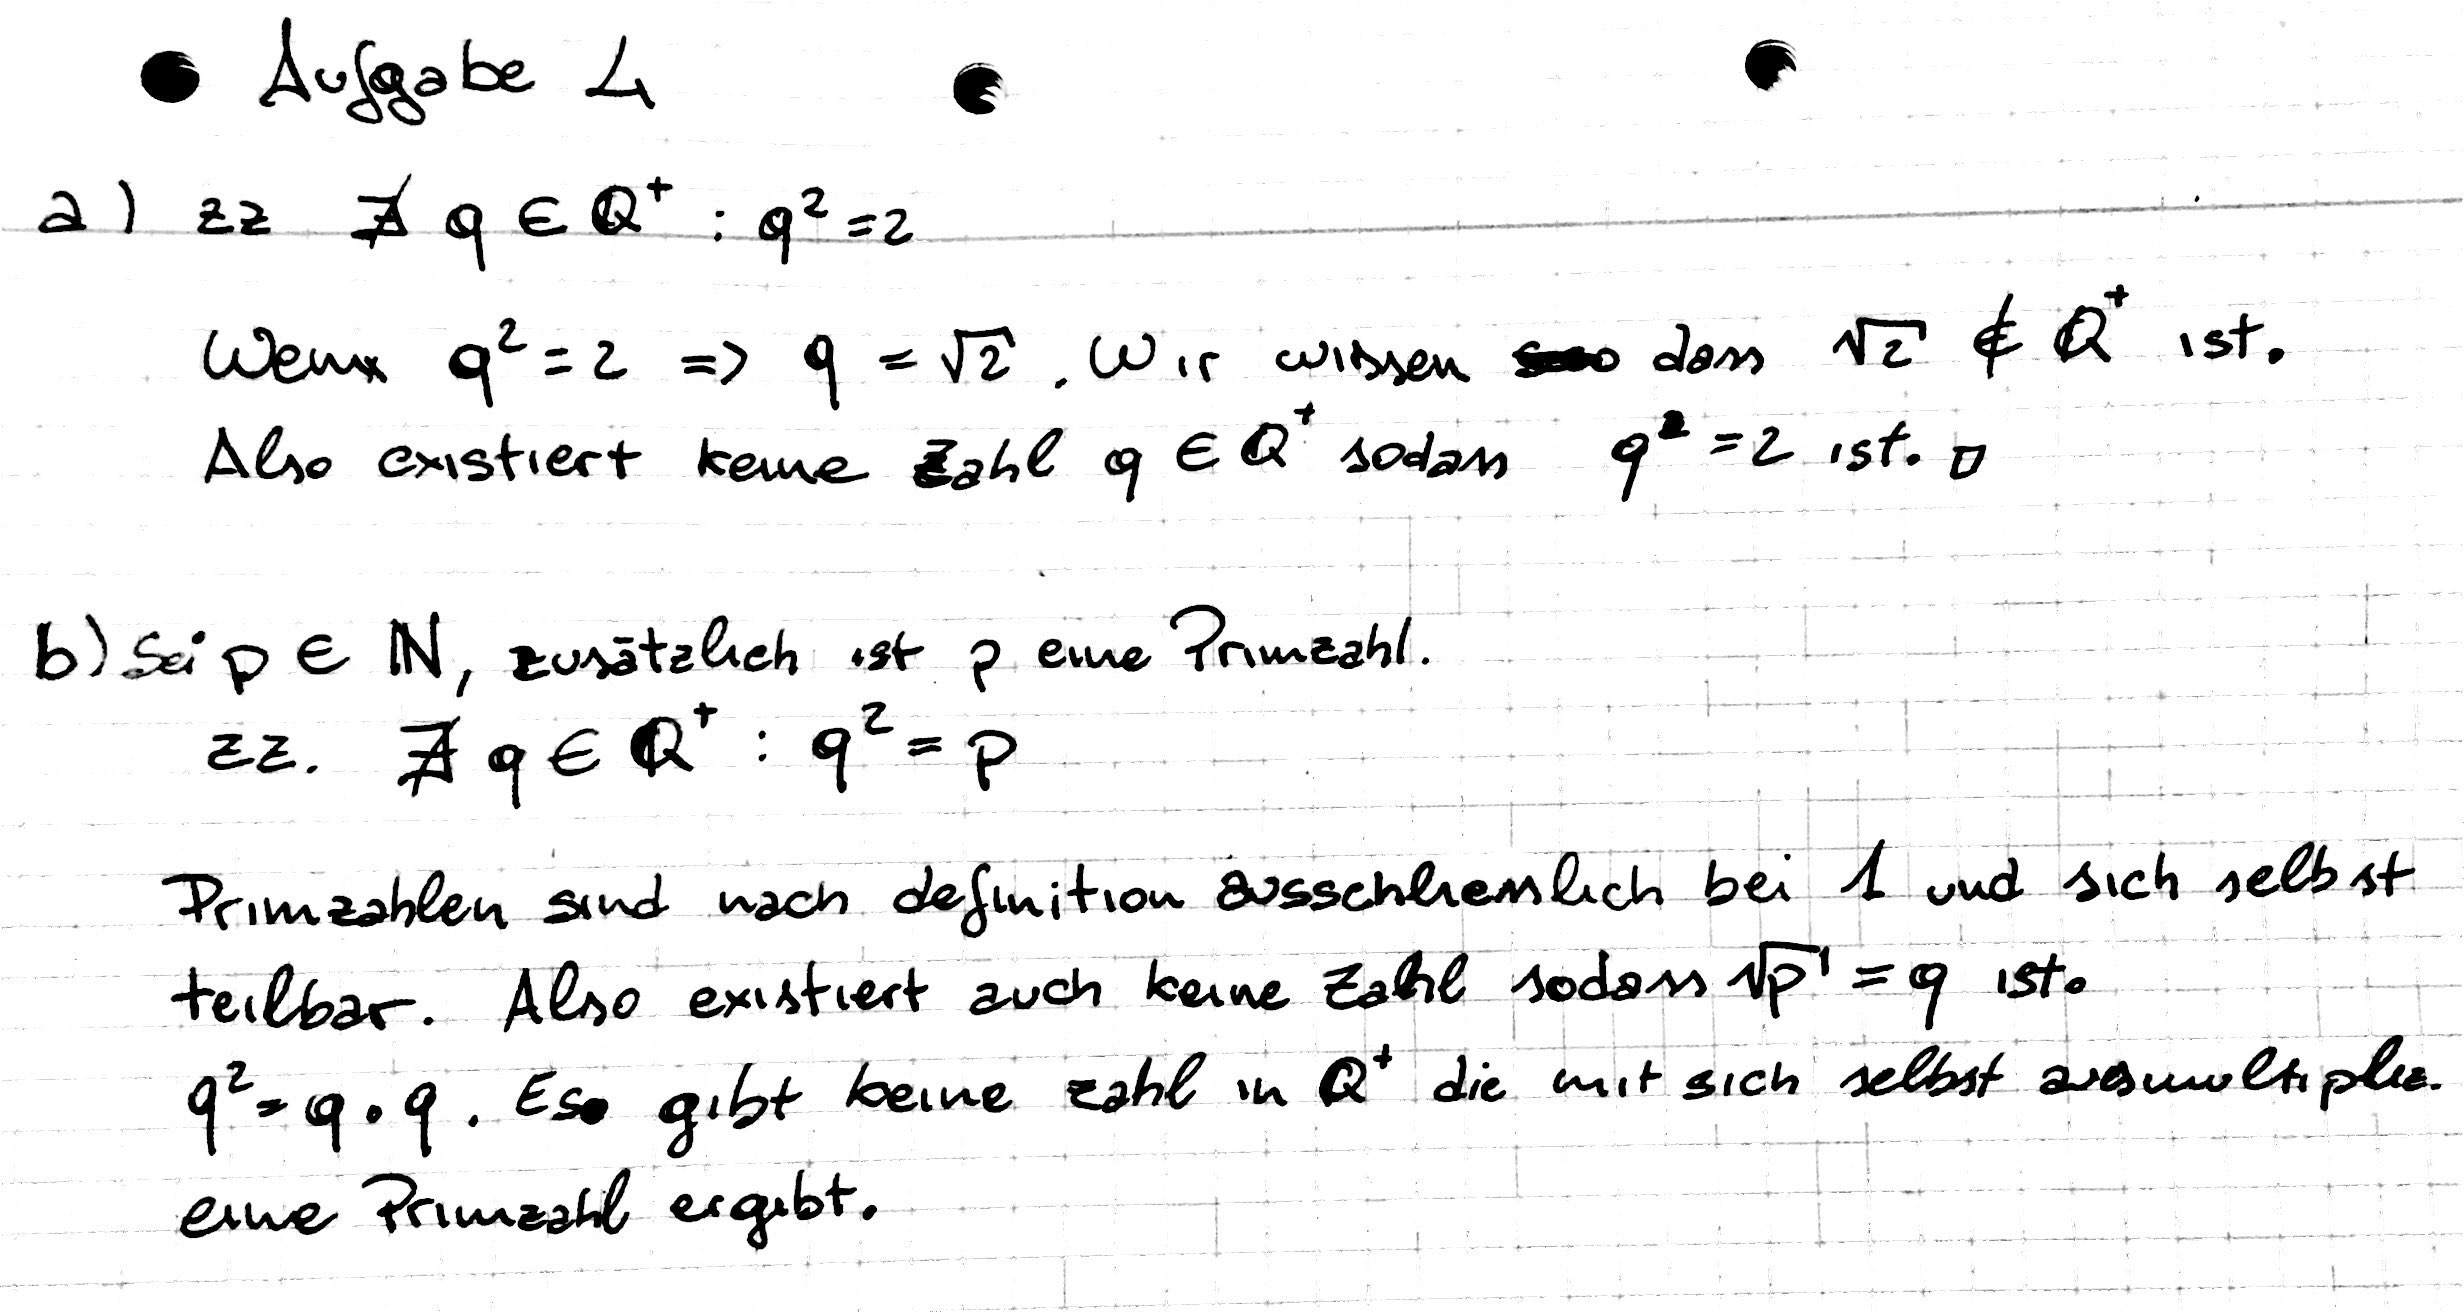
\includegraphics[scale=0.3]{AB1-4_1.jpg} 

\end{document}